\documentclass[UTF8]{ctexart}
\usepackage{subfigure}
\usepackage{caption}
\usepackage{amsmath,bm}
\usepackage{amssymb}
\usepackage{pifont}
\usepackage{geometry}
\usepackage{graphicx}
\usepackage{gensymb}
\usepackage{wrapfig}
\usepackage{titlesec}
\usepackage{float}
\usepackage{diagbox}
\usepackage{fancyhdr}
\usepackage{color}
\usepackage{bm}
\usepackage{siunitx}
\usepackage{ulem}
\usepackage{CJKulem}
\pagestyle{plain}
\geometry{a4paper,scale=0.8}
\CTEXsetup[format+={\raggedright}]{section} 
\title{固物2018期末答案}
\author{Deschain}
\titlespacing*{\section}
{0pt}{0pt}{0pt}
\titlespacing*{\subsection}
{0pt}{0pt}{0pt}
\titlespacing*{\paragraph}
{0pt}{0pt}{0pt}
\titlespacing*{\subparagraph}
{0pt}{0pt}{0pt}
\titleformat*{\section}{\normalsize}
\begin{document}
\maketitle
\section*{1.}
(1)\ding{172}X射线衍射/中子衍射/电子衍射\ding{173}中子非弹性散射/拉曼散射/布里渊散射/光子非弹性散射/X射线散射/X射线衍射(写出一种即可)\\
(2)\ding{172}电子的自旋磁矩\ding{173}电子的轨道磁矩\ding{174}电子的感生磁矩\ding{175}铁磁性\ding{176}亚铁磁性\ding{177}反铁磁性\ding{178}
正\ding{179}负\\
(3)\ding{172}匀加速\ding{173}晶格\\
(4)\ding{172}迁移率\ding{173}载流子浓度\ding{174}总掺杂\\
(5)\ding{172}$[-\frac{\pi}{2a},\frac{\pi}{2a}]$\ding{173}$\sqrt{15}:1$\\
(6)\ding{172}$24N_A$\ding{173}$16N_A$\ding{174}$8N_A$\ding{175}$\frac{4\pi}{G}$\\
(7)\ding{172}$-\frac{A}{r^6}$\ding{173}$\frac{B}{r^{12}}$\ding{174}$\sqrt[6]{\frac{2B}{A}}$\ding{175}$-\frac{NA^2}{8B}$\\
(8)\ding{172}$4.14\times10^{-15}J$\ding{173}$8.48\degree$\\
(9)\ding{172}$38.4cm/\Omega(\mu_n=300,\mu_p=150)$\\
(10)\ding{172}$-1.28\times10^{-5}m^3/C$\ding{173}$4.88\times10^{23}m^{-3}$\\
(11)\ding{172}$1.43\times10^{-24}m/s$\ding{173}$2.78\times10^{-15}$\ding{174}$3.98\times10^{-39}$\\
(12)\ding{172}独立\ding{173}统一\\
(13)\ding{172}球面\ding{173}$(3\pi^2n)^{\frac{1}{3}}$\ding{174}$\frac{\hbar^2}{2m}(3\pi^2n)^{\frac{2}{3}}$\ding{175}略低\\
\section*{2.)}
\begin{figure}[H]                                        
    \centering                                                
    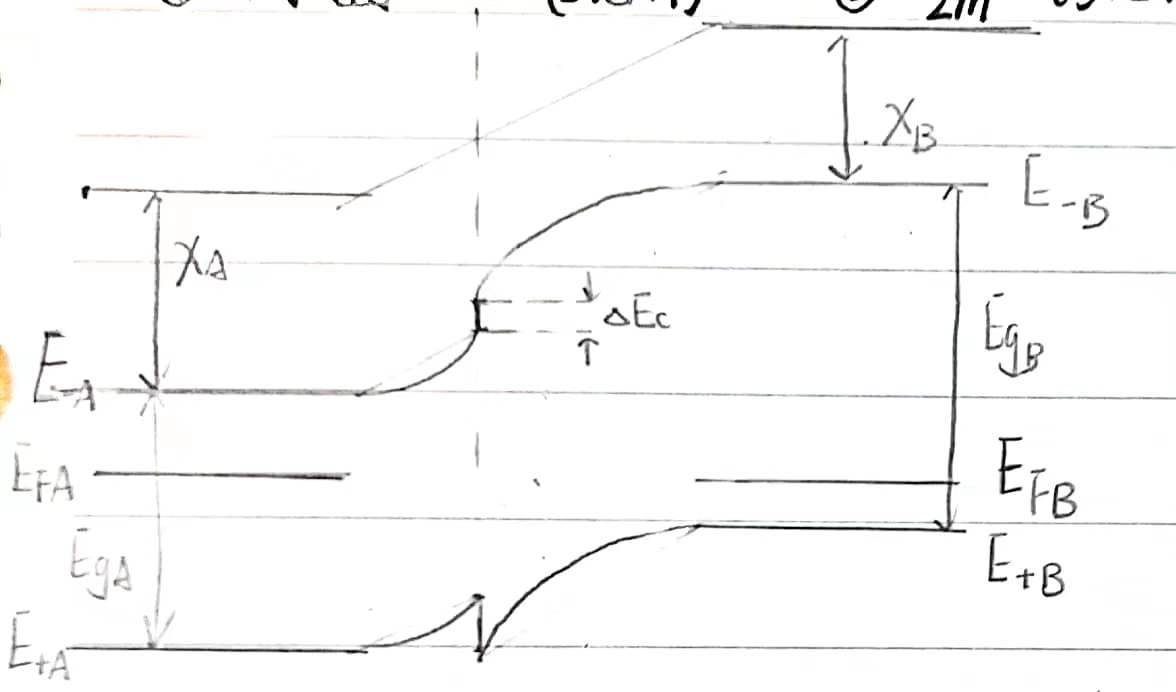
\includegraphics[width=7cm,height=4cm]{ans-2.jpg}        
    \caption*{}                                                                                   
\end{figure}
\begin{equation*}
    \begin{aligned}
        & \Delta E_C=\chi_A-\chi_B=0.17eV\\
        & \Delta E_V=\lvert \chi_A+E_{g_A}-(\chi_B+E_{g_B}) \rvert=0.3eV\\
        & V_D=\lvert \frac{1}{e}(E_{F_A}-E_{F_B}) \rvert=0.3V\\
    \end{aligned}
\end{equation*}
\section*{3.}
(1)
\begin{figure}[H]                                        
    \centering                                                
    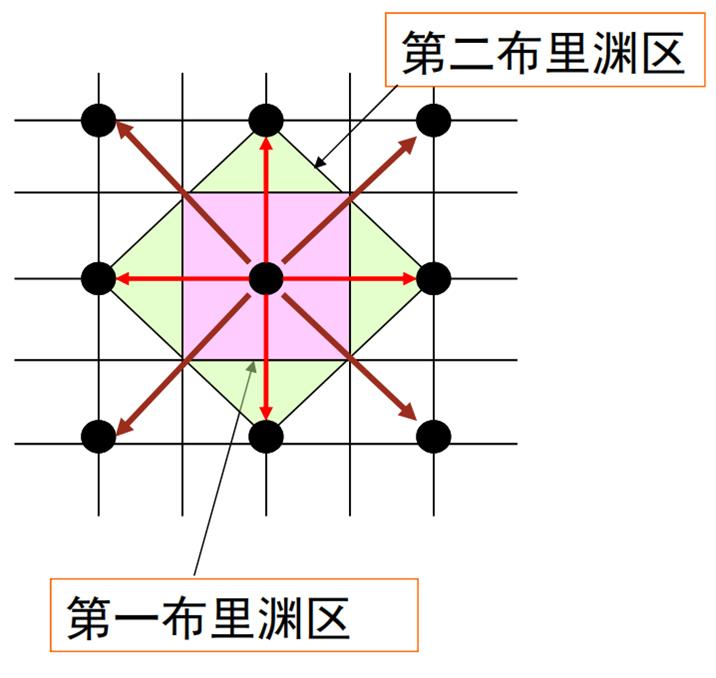
\includegraphics[width=4.5cm,height=4cm]{ans-3-1.jpg}        
    \caption*{}                                                                                   
\end{figure}
(2)
\begin{equation*}
    \begin{aligned}
       & k_F=\sqrt{2\pi n}=\sqrt{\frac{\pi}{2A^2}}\\ 
    \end{aligned}
\end{equation*}
(3)
\begin{figure}[H]                                        
    \centering                                                
    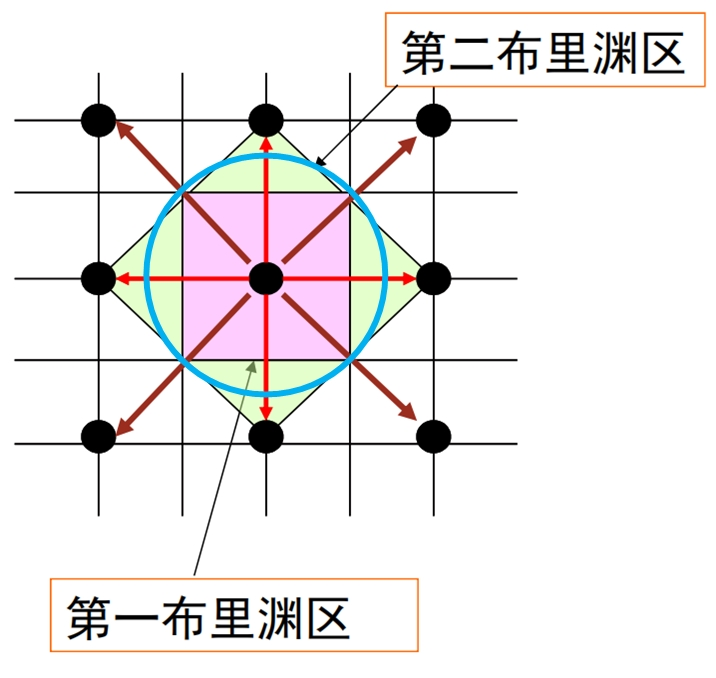
\includegraphics[width=4.5cm,height=4cm]{ans-3-3.jpg}        
    \caption*{}                                                                                   
\end{figure}
\section*{4.}
(1)
\begin{equation*}
    \begin{aligned}
        & n_{iSi}=(N_{-}N_{+})^{\frac{1}{2}}e^{-\frac{Eg_{Si}}{2k_BT}}=\frac{2}{h^3}(2\pi k_BT)^{\frac{3}{2}}
        (m_n^*m_p^*)^{\frac{3}{4}}e^{-\frac{Eg_{Si}}{2k_BT}}=9.40\times10^{11}cm^{-3}<N_D\\
        & n_{iGe}=(N_{-}N_{+})^{\frac{1}{2}}e^{-\frac{Eg_{Ge}}{2k_BT}}=\frac{2}{h^3}(2\pi k_BT)^{\frac{3}{2}}
        (m_n^*m_p^*)^{\frac{3}{4}}e^{-\frac{Eg_{Ge}}{2k_BT}}=2.15\times10^{14}cm^{-3}>N_D\\
    \end{aligned}
\end{equation*}
(2)
Si可以形成N结\\
(3)
\begin{equation*}
    \begin{aligned}
        & V_D=\frac{1}{e}(E_{Fn}-E_{Fp})=\frac{k_BT}{e}ln(\frac{N_DN_A}{n_{iSi}^2})=0.3745V\\
    \end{aligned}
\end{equation*}
\section*{5.}
(1)
\begin{equation*}
    \begin{aligned}
        &W(x) = \sum V_n e^{j\frac{2\pi n}{a}x}, V_n = \frac{1}{a}\int_{-\frac{a}{2}}^{\frac{a}{2}}W(x)e^{-j\frac{2\pi n}{a}x}dx 
        =\frac{2V_0}{a}cos(\frac{2\pi nb}{a})\\
        &V_{g_1} = \lvert 2V_1\rvert = \frac{4V_0}{a}cos(\frac{2b}{a}\pi), 
        V_{g_2} = \lvert 2V_2\rvert = \frac{4V_0}{a}cos(\frac{4b}{a}\pi)\\
    \end{aligned}
\end{equation*}
(2)$a>4b$不是导体,$a=4b$是导体。\\
(3)$a=8b$\\






\end{document}



